Nel caso precedente è stato automaticamente posto nullo il 
campo di spostamento elettrico all'esterno del condensatore, per
dimostrare ciò si suppone di avere uno strato piano di carica libera indefinito:
\begin{figure}[H]
\centering
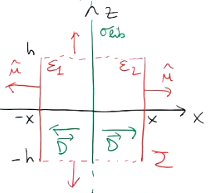
\includegraphics[width=0.3\linewidth]{lastra_piana_dielettrico}
\caption{Lastra piana carica}
\end{figure}
I due semipiani avranno costanti dielettriche differenti $\varepsilon_1$ 
ed $\varepsilon_2$.
Si studia il campo utilizzando la legge di Gauss:
$$
\oiint_{\Sigma} \vec{D}\cdot\hat{n}dS = Q_{lib}
$$
In questo caso si prende un parallelepipedo parallelo alle facce. La 
simmetria della distribuzione rispetto agli assi $y$ e $z$ fanno sì
che $\vec{D} = D_x(x)\vec{e}_x$ (in seguito $D_x$ sarà semplicemente $D$).

Applicando la legge di Gauss alla superficie $\Sigma$ si evince subito
che le superfici ortogonali ad $x$ non contribuiscono al flusso.
$$
\frac{\oiint_\Sigma \vec{D} \cdot \hat{n} dS }{hL}= -2\cancel{hL} D(-x) + 2\cancel{hL}D(x) = 
\sigma_{lib}\cancel{hL}
$$
Si evince la simmetria dispari del campo rispetto alla coordinata $x$ 
ossia $D(-x) = -D(x)$, sostituendo nella precedente si ottiene
$$
2D(x) = \sigma_{lib} \Rightarrow D(x) = \frac{\sigma_{lib}}{2}
$$
Il campo $\vec{D}$ è quindi pari in modulo e diretto in versi opposti
nei due semipiani. Per calcolare il campo $\vec{E}$ si potrà usare
la relazione costitutiva
$$
\vec{E} = \frac{\vec{D}}{\varepsilon}\Rightarrow
\begin{cases}
x > 0, & \vec{E}=\frac{\sigma_{lib}}{2\varepsilon_2} \vec{e}_x \\
x < 0, & \vec{E} = -\frac{\sigma_{lib}}{2\varepsilon_1} \vec{e}_x
\end{cases}\qquad
\begin{aligned}
\hat{n}\cdot(\vec{D}_2-\vec{D}_1) &= \sigma_{lib}\\
\hat{n}\cdot (\vec{E}_2-\vec{E}_1) &= \frac{\sigma_{lib}+\sigma_{pol}}{\varepsilon_0}
\end{aligned}
$$
Vale la continuità della componente normale di $\vec{D}$ ed $\vec{E}$.

\subparagraph{Condensatore piano con dielettrico}
Utilizzando il PSE
18:00




